\documentclass{article}

\usepackage{times}
\usepackage{geometry}
\geometry{a4paper,left=0.6cm,right=0.7cm,top=1.5cm,bottom=1cm,columnsep=0.8cm}

\usepackage{fontawesome}          % icônes de base seulement
\usepackage[hidelinks]{hyperref}
\usepackage{multicol}
\usepackage{tikz}
\usepackage{hyphsubst}
\usepackage{moresize}
\usepackage{hyphenat}
\usepackage{tabularx}
\usepackage{xcolor}
\usepackage{enumitem}
\usetikzlibrary{calc, positioning}
\newcolumntype{Y}{>{\RaggedRight\arraybackslash}X}

% icônes manquantes -> puce
\makeatletter
\@for\sym:=faBrain,faMicrochip,faHandshakeO,faTools,faNetworkWired,%
             faDatabase,faServer,faGit,faUsers,faComments,faCalendar,faGroup\do{%
  \@ifundefined{\sym}{\expandafter\newcommand\csname\sym\endcsname{\textbullet}}{}}
\makeatother

% couleurs
\definecolor{maincolor}{HTML}{f0fafc}
\definecolor{seccolor}{HTML}{ffffff}
\definecolor{gray}{HTML}{8c94a9}
\definecolor{sidetext}{HTML}{59cee5}

% bande latérale bleue
\usepackage{eso-pic}
\AddToShipoutPictureBG{%
  \begin{tikzpicture}[remember picture,overlay]
    \fill[maincolor] (current page.north west) rectangle
                     ([xshift=0.3\paperwidth] current page.south west);
  \end{tikzpicture}%
}

% listes
\setlist[itemize]{itemsep=-2pt,topsep=0pt,leftmargin=1.08cm}
\renewcommand{\labelitemi}{\textcolor{sidetext}{\footnotesize$\bullet$}}

\setlength{\parindent}{0pt}
\usepackage{paracol}
\columnratio{0.3}

\begin{document}
\pagestyle{empty}

\begin{paracol}{2}
% ────────────────────────────────────────
% Colonne gauche
% ────────────────────────────────────────
\color{sidetext}
\vspace*{-0.5cm}

\noindent
\begin{minipage}{\linewidth}
  \centering
  \begin{tikzpicture}
    \clip (0,0) circle (1.5cm) node[anchor=center]
      {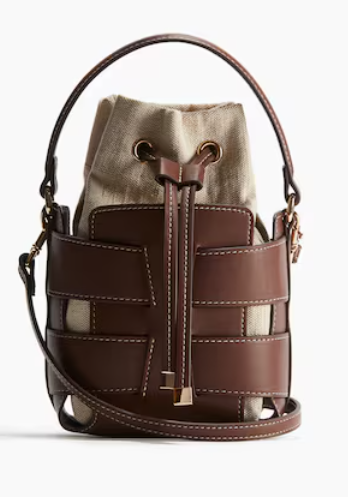
\includegraphics[width=3cm]{5e0a3ac70b9c4381b3f0eadaa8d926e6.png}};
  \end{tikzpicture}

  \vspace{3mm}
  {\color{black}\LARGE \textbf{Pape Saliou Fall}}

  \vspace{1mm}
  {\large Ingénieur Data Scientist \& Développeur IA}

  \vspace{3mm}
  {\color{gray}\rule{\linewidth}{0.4pt}} \\
\end{minipage}

% ── Coordonnées
\begin{tabular}{@{}c l}
  \faPhone &
  \begin{tabular}[t]{@{}l@{}}
    {\color{gray}Téléphone} \\ 0753481453
  \end{tabular} \\
  \\
  \faLinkedin &
  \begin{tabular}[t]{@{}l@{}}
    {\color{gray}LinkedIn} \\
    \href{https://www.linkedin.com/in/pape-saliou-fall-43154a211}{Mon LinkedIn}
  \end{tabular} \\
  \\
  \faMapMarker &
  \begin{tabular}[t]{@{}l@{}}
    {\color{gray}Adresse} \\ 95300 Pontoise \\ 
  \end{tabular} \\
  \\
  \faEnvelope &
  \begin{tabular}[t]{@{}l@{}}
    {\color{gray}Email} \\
    \href{mailto:papesalioufall2@gmail.com}{papesalioufall2@gmail.com}
  \end{tabular} \\
\end{tabular}

\vspace{2mm}
{\color{gray}\rule{\linewidth}{0.4pt}} \\

% ── Langues --------------------------------------------------------
{\color{black}{Langues}}

\vspace{2mm}
\begin{itemize}[leftmargin=*]
\item Français - \textcolor{gray}{Native}
\item Anglais - \textcolor{gray}{B2}\end{itemize}          % ← le placeholder va contenir \begin{itemize}…\end{itemize}

{\color{gray}\rule{\linewidth}{0.4pt}} \\

% ── Compétences ----------------------------------------------------
\vspace{2mm}
{\color{black}{Compétences Clés}}

\vspace{2mm}
\begin{itemize}[leftmargin=*]
\item Python
\item C
\item JavaScript
\item C++
\item R
\item SQL
\item PowerBI\end{itemize}              % ← idem, une vraie liste
\vspace{2mm}
{\color{gray}\rule{\linewidth}{0.4pt}} \\

% ── Centres d'intérêt
\vspace{2mm}
{\color{black}{Centres d’intérêt}}

\vspace{2mm}
\begin{itemize}[leftmargin=*]
\item Football
\item Natation
\item Lecture
\item Musique
\end{itemize}     % ← simple itemize ou tabular

\vfill
~

% ────────────────────────────────────────
\switchcolumn
% Colonne droite
% ────────────────────────────────────────
\color{black}

% ── Profil
\textcolor{black}{\Large \textbf{Profil Professionnel}} \\[2pt]
Data Scientist passionné d’intelligence artificielle, j’exploite la statistique avancée et le machine learning pour transformer des données complexes en solutions opérationnelles. Habitué à évoluer en autonomie comme en équipe, je conçois et déploie des plateformes data-driven du POC à la mise en production. Curieux et proactif, je recherche un environnement dynamique où l’innovation et l’excellence sont au cœur des projets. Mon objectif est d’apporter une valeur mesurable tout en relevant des défis technologiques stimulants. \\[8pt]

% ── Expérience
\textcolor{black}{\Large \textbf{Expérience Professionnelle}} \\[2pt]

\colorbox{maincolor}{%
  \begin{minipage}{\linewidth}
    \textbf{Data Scientist \& Développeur IA} \\ Prepaya \\ 01/2024 – Présent
    \begin{itemize}
      \item Conçu et déployé une plateforme d’IA cloud-native avec Python et PostgreSQL, améliorant l’accessibilité des modèles prédictifs. \item Implémenté des algorithmes de machine \& deep learning pour l’analyse de séries temporelles, augmentant la précision des prévisions. \item Industrialisé les solutions via API Flask et déploiement Heroku, réduisant le délai de mise en production.
    \end{itemize}
  \end{minipage}}

\vspace{3mm}


\colorbox{maincolor}{%
  \begin{minipage}{\linewidth}
    \textbf{Apprenti Risk Analyst \& Data Scientist} \\ AXA XL (Groupe AXA) \\ 12/2022 – 12/2023
    \begin{itemize}
      \item Automatisé la collecte et l’intégration des données financières avec Python et VBA, divisant par deux le temps de traitement mensuel. \item Développé des tableaux de bord Power BI pour la facturation, offrant une visibilité temps réel aux équipes finance et management. \item Créé des modèles prédictifs de sinistres en R/Python, aidant à estimer la probabilité de survenance et optimiser la tarification.
    \end{itemize}
  \end{minipage}}

\vspace{3mm}


\colorbox{maincolor}{%
  \begin{minipage}{\linewidth}
    \textbf{Apprenti Data Scientist} \\ Prepaya \\ 09/2021 – 08/2022
    \begin{itemize}
      \item Déployé des modèles NLP (BERT, T5) pour générer automatiquement des formulaires, accélérant la production documentaire. \item Mené une analyse de sentiments sur les retours clients, fournissant des indicateurs clés de satisfaction aux équipes produit. \item Réalisé du web scraping et de l’automatisation (BeautifulSoup, Selenium) afin d’enrichir et fiabiliser les corpus textuels.
    \end{itemize}
  \end{minipage}}   % ← blocs \colorbox{maincolor}{\begin{minipage}…}

\vspace{8mm}

% ── Formation
\textcolor{black}{\Large \textbf{Formation}} \\[2pt]

    \begin{tabularx}{\linewidth}{@{}c X@{}}
    \textcolor{sidetext}{\faGraduationCap} &
    \textbf{Master 2 Data Science} \\
    & Sorbonne Université, Paris \\
    & \begin{itemize}[leftmargin=*]
  \item Analyse de données, machine learning et deep learning appliqués à de grands ensembles de données. \item Statistiques avancées, séries chronologiques et modèles structurels latents. \item Pratique de bases de données et calcul parallèle pour le traitement intensif.
\end{itemize} \\
    & \textit{09/2021 – 03/2022}
    \end{tabularx}
           % ← lignes tabular par diplôme

\end{paracol}
\end{document}

